\documentclass{beamer}
    \usefonttheme{serif}
\usepackage{subcaption}
\usepackage[backend=biber,sortcites,maxcitenames=1,maxbibnames=2]{biblatex}
    \addbibresource{./references.bib}
\usepackage{adjustbox}
\usepackage{tikz}
\usetikzlibrary{
  positioning,
  arrows.meta,
  shapes.geometric
}

\title[Tokenization Effects]{Tokenization Effects in Multilingual LLMs}
\author{Gustaf Gren}
\date{Project Proposal}

\begin{document}

% -----------------------
\begin{frame}
  \titlepage
\end{frame}

% -----------------------
\begin{frame}{Aim}

This thesis aims to shed light on how tokenization choices influence
representations, robustness, and cross-lingual performance in multilingual
models using \texttt{TokSuite} \parencite{altintas2025}, LLMs trained
identically except for the choice in tokenizer.

\end{frame}

% -----------------------
\begin{frame}{Tokenization \& Robustness}
\begin{itemize}
  \item LLMs uses subword tokenization (e.g. BPE)
  \item Same text can have multiple valid tokenizations
  \item LLMs are trained on only canonical tokenization, yet LLMs remain surprisingly robust.
\end{itemize}

{
\footnotesize
\begin{figure}[h]
\centering

\begin{subfigure}[t]{0.45\textwidth}
\centering
\begin{tabular}{|c|c|}
\hline
\textbf{bow} & \textbf{ling} \\
\hline
8176 & 1359 \\
\hline
\end{tabular}
\caption{Canonical tokenization}
\end{subfigure}

\begin{subfigure}[t]{0.45\textwidth}
\centering
\begin{tabular}{|c|c|c|}
\hline
\textbf{b} & \textbf{ow} & \textbf{ling} \\
\hline
65 & 322 & 1359 \\
\hline
\end{tabular}
\caption{Non-canonical tokenization}
\end{subfigure}

\begin{subfigure}[t]{0.45\textwidth}
\centering
\begin{tabular}{|c|c|}
\hline
\textbf{bow} & \textbf{king} \\
\hline
8176 & 3364 \\
\hline
\end{tabular}
\caption{Surface level perturbation}
\end{subfigure}


\caption{Demonstrating canonical vs.\ a possible non-canonical tokenization and perturbation example for the word `bowling' using GPT2-tokenizer.}
\label{fig:noncanon}
\end{figure}

}
\end{frame}

% -----------------------
\begin{frame}{Mechanistic Interpretability}

\textit{How do we uncover the ``black box'' in LLMs?}

\end{frame}

% -----------------------
\begin{frame}{Mechanistic Interpretability \& Multilinguality}
Multilingual models show layered language processing, with language-specific processing occurring in early-to-middle layers, and late layers.

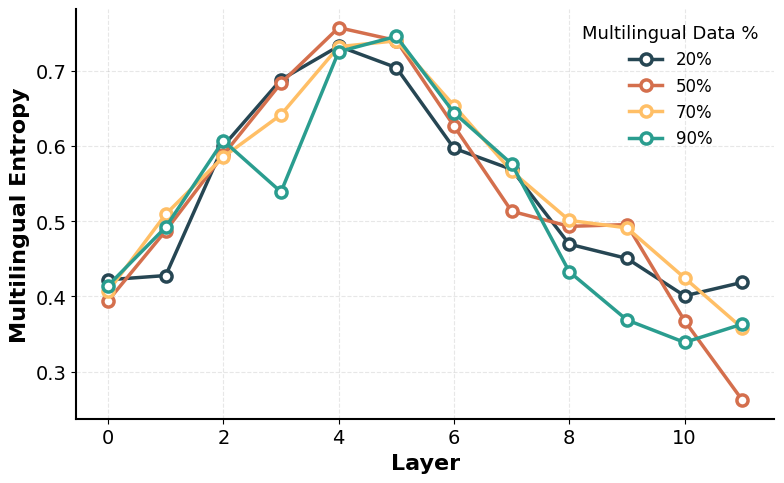
\includegraphics[width=0.8 \linewidth]{img/harasse2025_img.png} \\
``language-agnosticity'' / layer \parencite{harrasse2025}
\end{frame}

% -----------------------
\begin{frame}{Mechanistic Interpretability \& Tokens = True?}

Similarly, \textcite{kaplan2025} suggests early-to-middle layers
\textit{\textbf{detokenize}} into a model-internal vocabulary.

\end{frame}

% -----------------------
\begin{frame}{Detokenization}
\begin{columns}
\column{0.5\textwidth}
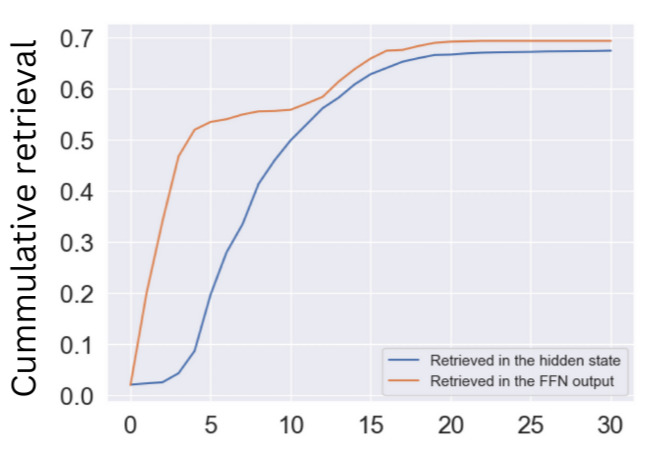
\includegraphics[width=0.9\linewidth]{img/kaplan_word_retreival.jpeg}

\column{0.5\textwidth}
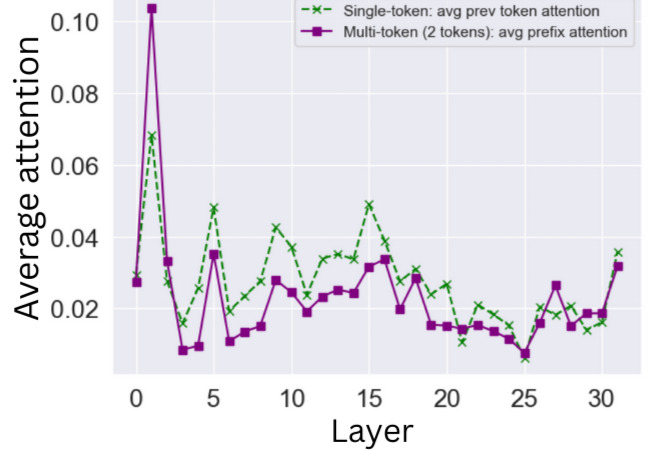
\includegraphics[width=0.9\linewidth]{img/kaplan_attention.jpeg}
\end{columns}
\end{frame}

% -----------------------
\begin{frame}{Detokenization gaps}

\textcite{kaplan2025} limit their analysis to English and don't perform comparisons between tokenizers.

\end{frame}

\begin{frame}{Research Questions}
\begin{itemize}
\item[\textbf{RQ1}] Do multilingual models exhibit detokenization patterns
across languages and tokenizers? How do patterns differ between more
monolingual (e.g.  GPT-2) and more multilingual tokenizers (e.g. BLOOM)?
\end{itemize}
\end{frame}

% -----------------------
\begin{frame}{Tokenization alignment/overlap}
\begin{itemize}
  \item Tokenization compression ratios affects performance and transfer,
  generally more compression = better performance \parencite{ahia2023}.
  \item However, more overlapping/aligned vocabularies leads to increased
  performance \parencite{kallini2025, limisiewicz2023}.
  \item Cross-lingual tokenization effects are poorly understood.
\end{itemize}
\end{frame}

% -----------------------
\begin{frame}{Research Questions}
\begin{itemize}

\item[\textbf{RQ1}] Do multilingual models exhibit detokenization patterns
across languages and tokenizers? How do patterns differ between more
monolingual (e.g.  GPT-2) and more multilingual tokenizers (e.g. BLOOM)?

\item[\textbf{RQ2}] Do majority, minority, and out-of-training languages show
different processing patterns under tokenization perturbations?

\item[\textbf{RQ3}] Does higher token alignment scores lead to an increase in
robustness and performance on NLU benchmarks across tokenizers?

\end{itemize}
\end{frame}

% -----------------------
\begin{frame}{Methodology}
\begin{itemize}
\item  \texttt{TokSuite} models \parencite{altintas2025}, trained identically except for tokenizer.
\item For each selected tokenizer and language:
\end{itemize}
\begin{adjustbox}{max width=\textwidth}

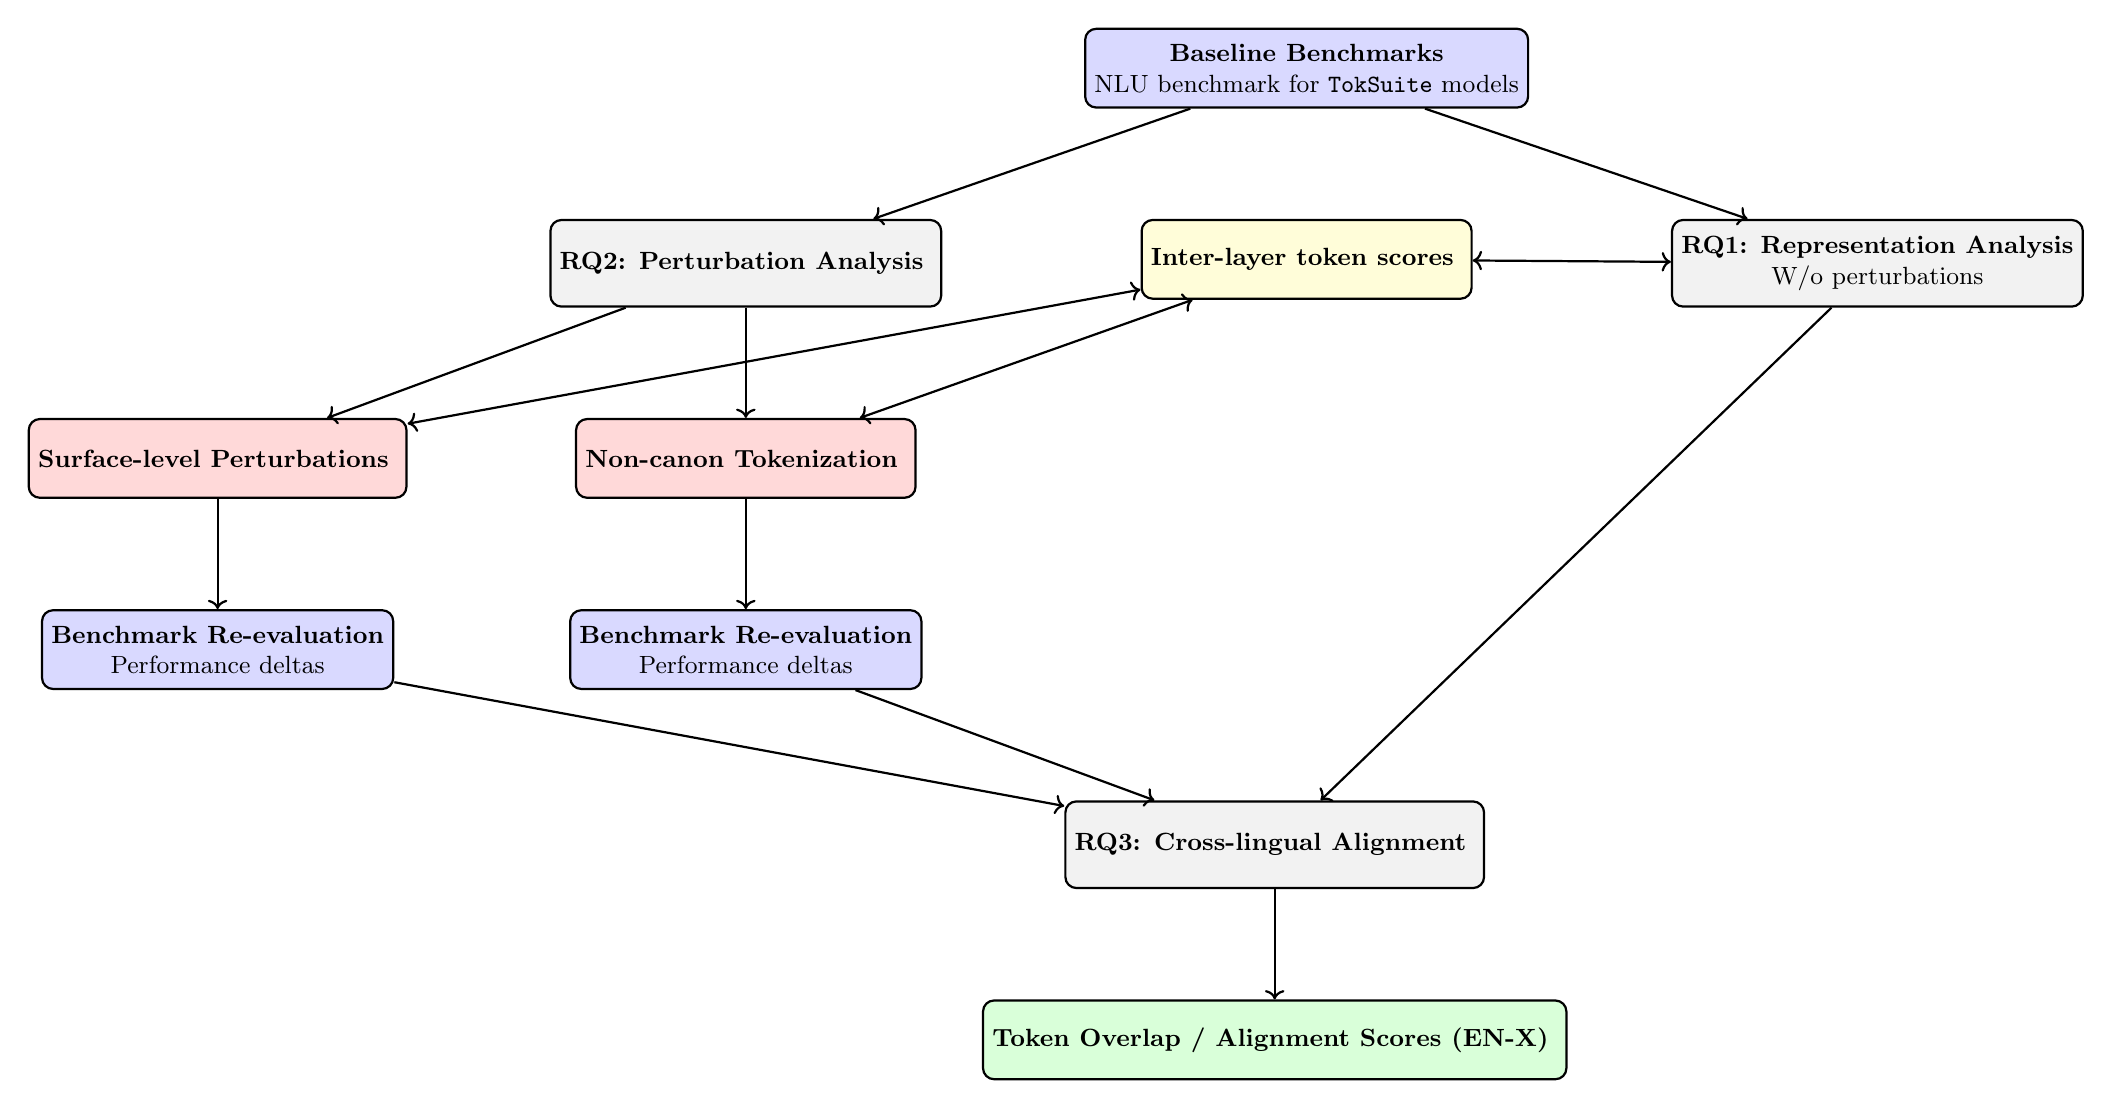
\begin{tikzpicture}[
    node distance=1.4cm and 1.8cm,
    every node/.style={font=\small},
    box/.style={
        rectangle,
        rounded corners,
        draw=black,
        thick,
        align=center,
        minimum width=3.8cm,
        minimum height=1.1cm,
        fill=gray!10
    },
    benchbox/.style={
        rectangle,
        rounded corners,
        draw=black,
        thick,
        align=center,
        minimum width=3.8cm,
        minimum height=1.0cm,
        fill=blue!15
    },
    layerbox/.style={
        rectangle,
        rounded corners,
        draw=black,
        thick,
        align=center,
        minimum width=3.8cm,
        minimum height=1.0cm,
        fill=yellow!15
    },
    alignbox/.style={
        rectangle,
        rounded corners,
        draw=black,
        thick,
        align=center,
        minimum width=3.8cm,
        minimum height=1.0cm,
        fill=green!15
    },
    pertbox/.style={
        rectangle,
        rounded corners,
        draw=black,
        thick,
        align=center,
        minimum width=3.8cm,
        minimum height=1.0cm,
        fill=red!15
    },
    arrow/.style={->, thick},
    doublearrow/.style={<->, thick}
]

% Top benchmark (baseline)
\node[benchbox] (bench0) {%
\textbf{Baseline Benchmarks} \\
NLU benchmark for \texttt{TokSuite} models
};

% RQ blocks
\node[box, below right=of bench0] (rq1) {%
\textbf{RQ1: Representation Analysis}\\
W/o perturbations
};

\node[box, below left=of bench0] (rq2) {%
\textbf{RQ2: Perturbation Analysis}
};

\node[pertbox, below left=of rq2] (typo) {%
\textbf{Surface-level Perturbations}
};

\node[pertbox, below=of rq2] (noncanon) {%
\textbf{Non-canon Tokenization}
};

\node[benchbox, below=of typo] (bench2typo) {%
\textbf{Benchmark Re-evaluation}\\
Performance deltas
};

\node[benchbox, below=of noncanon] (bench2noncanon) {%
\textbf{Benchmark Re-evaluation}\\
Performance deltas
};

\node[layerbox, below=of bench0] (tokenscores) {%
\textbf{Inter-layer token scores}
};

\node[box, below right=of bench2noncanon] (rq3) {%
\textbf{RQ3: Cross-lingual Alignment}
};

\node[alignbox, below=of rq3] (alg) {%
\textbf{Token Overlap / Alignment Scores (EN-X)}
};

% Arrows
\draw[arrow] (bench0) -- (rq1);
\draw[arrow] (bench0) -- (rq2);
\draw[doublearrow] (rq1) -- (tokenscores);
\draw[doublearrow] (typo) -- (tokenscores);
\draw[doublearrow] (noncanon) -- (tokenscores);
\draw[arrow] (rq1) -- (rq3);
\draw[arrow] (rq2) -- (typo);
\draw[arrow] (rq2) -- (noncanon);
\draw[arrow] (typo) -- (bench2typo);
\draw[arrow] (noncanon) -- (bench2noncanon);
\draw[arrow] (bench2typo) -- (rq3);
\draw[arrow] (bench2noncanon) -- (rq3);
\draw[arrow] (rq3) -- (alg);

\end{tikzpicture}
\end{adjustbox}
\end{frame}

\begin{frame}[allowframebreaks]{References}
\printbibliography
\end{frame}

\end{document}
